\subsection{Actividades Realizadas}

\subsubsection{Selección de Footprints}

Para comenzar el desarrollo de la PCB, primero se tomó la lista de componentes de la plataforma, provista por el programa, y se le asignó a cada uno de los componentes una \textit{footprint}, que es el patrón de pads (para dispositivos de montaje superficial o SMD) u orificios (para dispositivos de tecnología \textit{through-hole} o THT) de un componente sobre la superficie de la placa, sobre el cuál luego se suelda el componente apropiado.\\ 

Para esta plataforma se decidió utilizar, siempre que fuese posible, componentes de tipo SMD, ya que estos no atraviesan la placa y facilitan el ruteo de pistas de cobre al no ocupar espacio en la capa opuesta de la placa. Casi todas las resistencias y capacitores que se utilizan en la placa son de montaje superficial, de dimensiones 1206 (\SI[]{3}[]{\milli\metre} x \SI[]{1.5}[]{\milli\metre}), ya que es un tamaño bastante reducido que es fácil de conseguir en proveedores locales. En la figura \ref{fig:encapsulados} se puede ver este junto con otros encapsulados utilizados en la plataforma.\\

\begin{figure}[h]
    \centering
    \begin{subfigure}
        \centering
        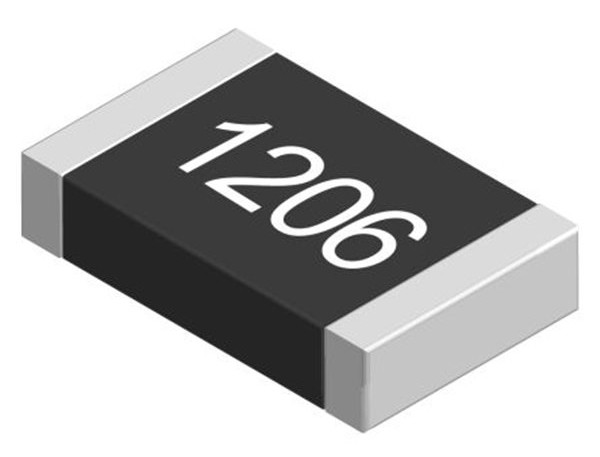
\includegraphics[scale=0.4]{Imagenes/1206.jpg}
    \end{subfigure}
    \hspace{1em}
    \begin{subfigure}
        \centering
        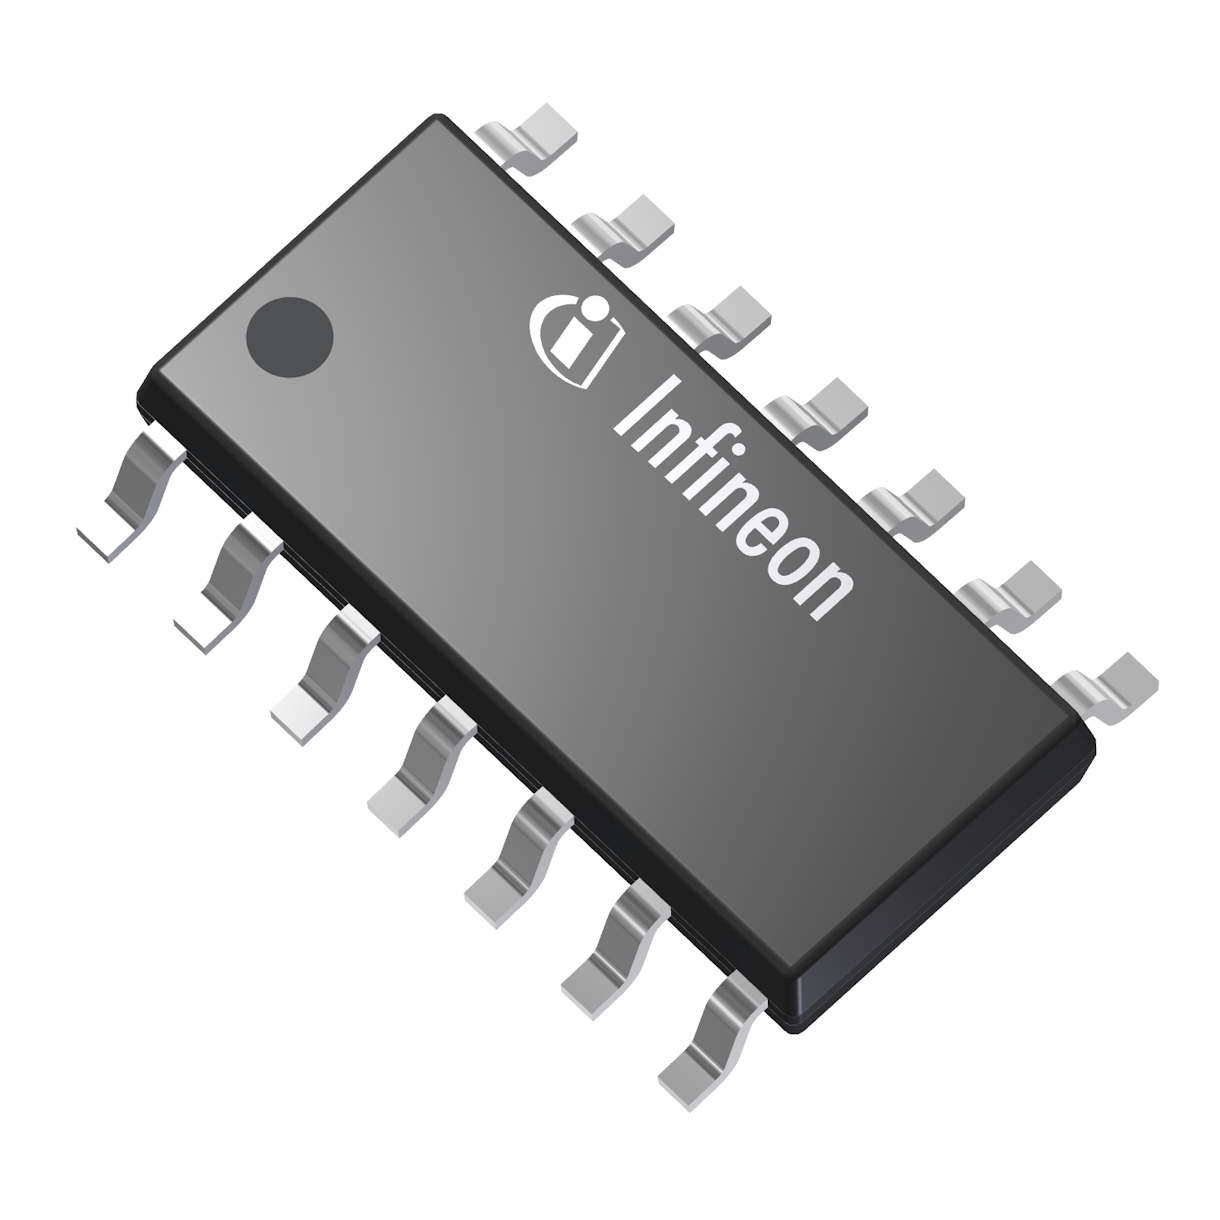
\includegraphics[scale=0.05]{Imagenes/Driver DSO-14.png}
    \end{subfigure}
    \hspace{1em}
    \begin{subfigure}
        \centering
        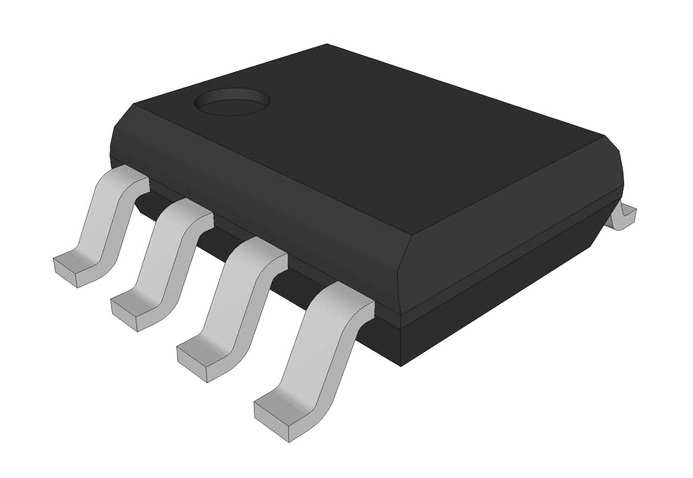
\includegraphics[scale=0.3]{Imagenes/SOIC8.jpg}
    \end{subfigure}
    \hspace{1em}
    \begin{subfigure}
        \centering
        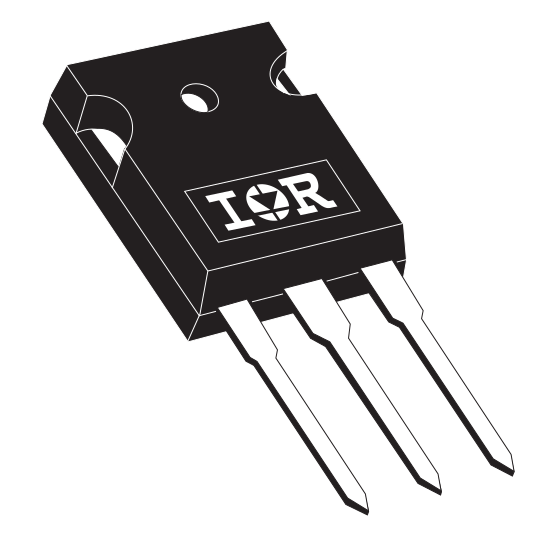
\includegraphics[scale=0.1]{Imagenes/IRFP150-TO247AC.png}
    \end{subfigure}
    \hspace{1em}
    \begin{subfigure}
        \centering
        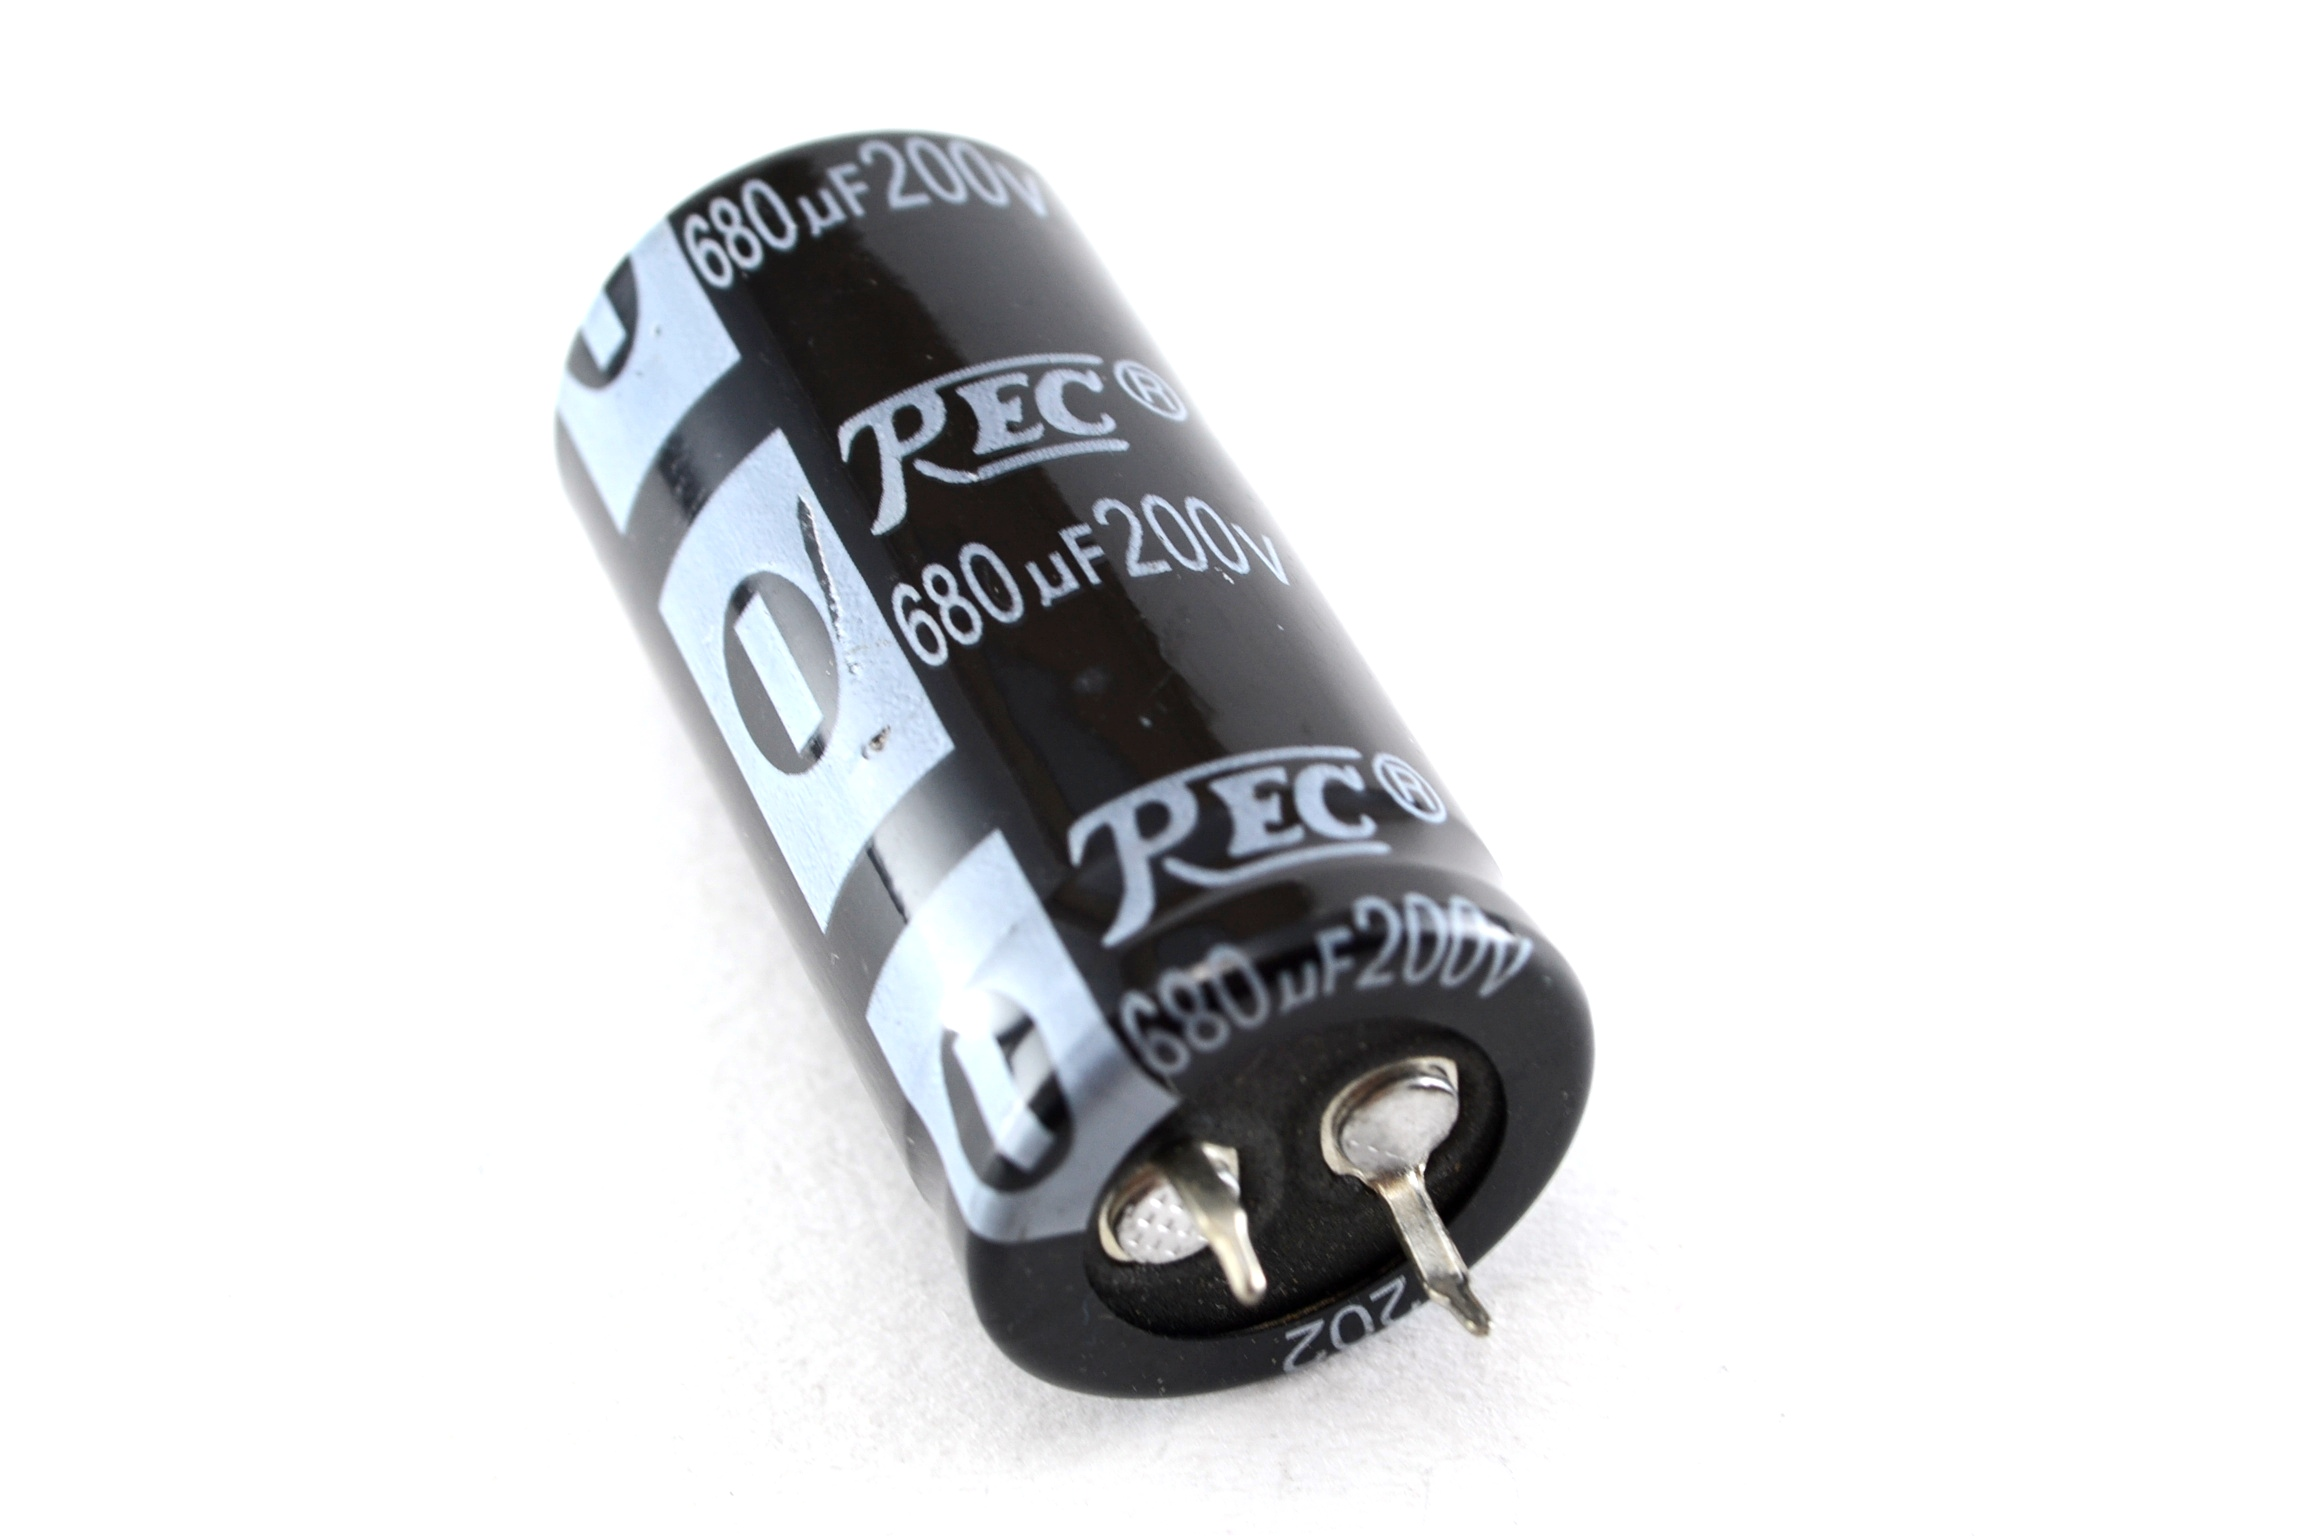
\includegraphics[scale=0.18]{Imagenes/Capacitor Blindado.jpg}
    \end{subfigure}
    \caption{Algunos de los encapsulados que utilizan los componentes de la placa de circuito impreso. Componentes fuera de escala.}
    \label{fig:encapsulados}
\end{figure}

Para esto se comenzó utilizando la biblioteca de footprints y componentes disponible por defecto en el programa. Pero rápidamente se hizo claro que esto es insuficiente, por lo que se tuvo que recurrir a páginas web como \textit{SnapEDA}, que tiene un catálogo gratuito de footprints y símbolos esquemáticos para una enorme cantidad de componentes electrónicos.\\

\subsubsection{Posicionamiento y Conexión de Footprints}
 
Una vez seleccionadas todas las footprints necesarias, se posicionaron las mismas de la manera más compacta posible en las dos capas de cobre disponible, dando suficiente espacio para luego poder rutear las pistas de cobre que conectan los distintos componentes del sistema. Para esto se tuvo en cuenta que la plataforma cuenta con tres distintas puestas a tierra: GND\textsubscript{1} para el lado primario del convertidor, GND\textsubscript{2} para el lado secundario, y GND\textsubscript{D} para las partes digitales y de señal. Esto se realiza con el propósito de aislar las partes de señal de la plataforma, más sensibles al ruido, de las partes de potencia más ruidosas, además de proteger a los circuitos sensibles de posibles picos de tensión y corriente.\\

Para el caso de los circuitos integrados, como el sensor LM5056A o el aislador de señal ISO7242C, se siguieron las recomendaciones de los fabricantes encontradas en las hojas de datos, que establecen guías de posicionamiento y conexión de componentes auxiliares, como capacitores y resistencias, respecto a los dispositivos (por ejemplo, los capacitores de bypass de los pines de alimentación deben estar lo más cerca posible del integrado).\\

\paragraph{Trazado y Dimensionamiento de Pistas}

Una vez ordenados los componentes (separados apropiadamente según la puesta a tierra que le corresponde), se procedió a hacer el trazado o ruteo de las pistas de cobre que interconectan todos los distintos componentes, al mismo tiempo que se decidía por la dimensión de las mismas.\\

Todas las pistas de cobre en la PCB se dimensionaron según la ecuación establecida por la norma IPC-2221, que permite calcular el ancho $W$ (en \unit{\milli\metre}) necesario para una que una pista de cobre de grosor $H$ (en \unit{\milli\metre}) con una corriente circulante $I$ (en \unit{\ampere}) no eleve su temperatura más de $\Delta T$ grados centígrados.

\begin{equation}\label{eq:IPC2221}
    I = \num{0.048}\cdot (\Delta T)^{\num{0.44}}\cdot (\num{1550}\cdot W\cdot H)^{\num{0.725}}
\end{equation}

En este caso, se eligió un grosor $H$ fijo de \SI[]{0.035}[]{\milli\metre} con una máxima elevación de temperatura $\Delta T$ de \SI[]{20}[]{\celsius}. Entonces, reemplazando la corriente por el máximo valor de corriente que puede circular por una pista, se puede despejar su ancho mínimo $W$ en \unit{\milli\metre}.\\

En el caso de las tres puestas a tierra, se utilizó la funcionalidad \textit{fill zone} o rellenar zona en lugar de utilizar pistas individuales, principalmente por sus beneficios en disipación térmica del calor generado por las altas corrientes, además de mejorar la inmunidad electromagnética del sistema. Esta funcionalidad permite elegir una zona de una o varias capas de cobre y rellenarla con cobre en todas las partes en las que no haya una pista preexistente, para luego conectar todos los terminales correspondientes a una de las tierras a este plano de cobre.\\

Siempre se intenta mantener las pistas, en especial las de altas corrientes, en la misma capa de cobre. En caso de no ser posible, ya sea por componentes que se interponen en el camino u otras razones, se utilizan \textit{vías PTH}, que son perforaciones en la placa con sus paredes recubiertas por material conductor, que permiten conectar eléctricamente pistas en distintas capas de cobre.\\

\subsubsection{Verificación del Diseño}
 
Con los componentes organizados y conectados mediante pistas de cobre, se obtuvo una versión preliminar de la placa de circuito impreso doble capa de dimensiones de \SI[]{15}[]{\centi\metre} x \SI[]{16}[]{\centi\metre}. Pero, previo a generar los archivos de fabricación definitivos, se realizó una verificación del diseño e implementación de la plataforma en la PCB, utilizando la funcionalidad DRC (\textit{Design Rules Checker} o Verificador de Reglas de Diseño). Esta funcionalidad permite ingresar las tolerancias y límites de fabricación, como por ejemplo la mínima distancia entre pistas, y al ejecutar la herramienta el programa indica los lugares de la PCB en los cuáles se está debajo de la mínima tolerancia de fabricación.\\

En este caso, se eligió el fabricante de placas de circuito impreso Mayer Circuitos Impresos, de origen nacional, radicado en la ciudad de Buenos Aires. Según lo especificado, este fabricante tiene tolerancias de fabricación suficientemente bajas, con las más importantes presentadas a continuación: separación mínima entre pistas y ancho mínimo de pistas de \SI[]{0.15}[]{\milli\metre}, separación mínima entre agujeros de \SI[]{0.2}[]{\milli\metre}, ancho mínimo de pads THT de \SI[]{0.3}[]{\milli\metre}, ancho mínimo de pads SMD de \SI[]{0.25}[]{\milli\metre}, separación mínima entre pads (para máscara anti-soldadura) de \SI[]{0.2}[]{\milli\metre}.\\

\subsubsection{Contacto con Fabricantes}
 
Con el diseño de la plaqueta finalizado y verificado, se generaron los archivos de fabricación \textit{Gerber} finales, con los que los fabricantes pueden producir las PCB. Entonces, se contactó por medio de correo electrónico al fabricante elegido, Mayer Circuitos Impresos, buscando un presupuesto para establecer el valor de la fabricación. Con el presupuesto obtenido, se enviaron los archivos obtenidos previamente para que se pudiera comenzar el proceso de elaboración, con un tiempo estimado para completar el proceso de un mes.\\